\section{Графы. Способы их представления в памяти компьютера. Матрицы смежости, матрицы инцедентности, списки связности, представление на двух массивах (CSR).}

На протяжении всего билета будем рассматривать граф на иллюстрации ниже

\begin{figure}[h!]
	\centering
	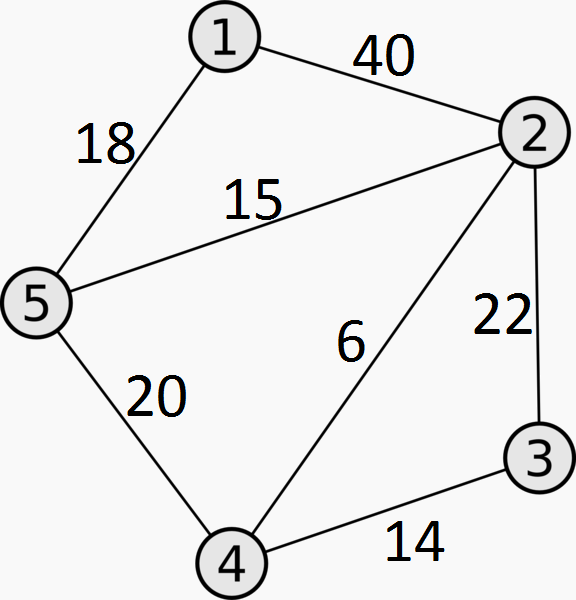
\includegraphics[width=0.4\linewidth]{img_easy/5_1.png}
	\captionsetup{labelformat=empty}
	\caption{}
	\label{fig:51}
\end{figure}

\subsection{Матрица смежности}

\begin{definition}
	Матрица смежности --- 
\end{definition}

\subsection{Матрица инцидентности}

\subsection{Списки смежности}

\subsection{CSR}